\documentclass[10pt]{beamer}
\usepackage[utf8]{inputenc}
\usetheme[sectionpage=none,
    subsectionpage=progressbar,
    progressbar=frametitle,
    numbering=fraction,
    block=fill]{metropolis}
\usepackage{xcolor}

\makeatletter
\setlength{\metropolis@titleseparator@linewidth}{2pt}
\setlength{\metropolis@progressonsectionpage@linewidth}{2pt}
\setlength{\metropolis@progressinheadfoot@linewidth}{2pt}
\makeatother

\usepackage{pgfplots}
\pgfplotsset{width=7cm,compat=1.8}

\usepackage{smartdiagram}
\usesmartdiagramlibrary{additions}
\definecolor{fajny_szary}{HTML}{716b58}
\definecolor{fajny_bar}{HTML}{c2b385}

\setbeamercolor{progress bar}{fg=fajny_bar}
\setbeamercolor{frametitle}{fg=white, bg=fajny_szary}

\usepackage{lipsum}% http://ctan.org/pkg/lipsum
\usepackage{hanging}% http://ctan.org/pkg/hanging
\setbeamertemplate{footnote}{%
  \hangpara{2em}{1}%
  \makebox[2em][l]{\insertfootnotemark}\footnotesize\insertfootnotetext\par%
}

\usepackage{polski}
\usepackage[polish]{babel}
\usepackage{setspace,amsmath,booktabs}

\title[]{Współczesne rozwiązania technologiczne pomagają w rozwoju i edukacji}
\author[A.~Greloch \and W.~Zaremba \and M.~Zwierzyński \and J.~Lipski \and K.~Szturemski]{A.~Greloch \and W.~Zaremba \and M.~Zwierzyński \and J.~Lipski \and K.~Szturemski}
\institute[G1PIA] % (optional)
{
  Klasa 3j\\
  Gimnazjum nr. 1 im. Powstańców Warszawy w Piasecznie
}
\date{Piaseczno, 16 maja 2018}

\begin{document}

\frame{\titlepage}

\section{Problem}
\subsection{Wprowadzenie do problematyki projektu}
\setcounter{subsection}{1}

\renewcommand{\arraystretch}{1.2}
\setstretch{1.1}

\begin{frame}
  \frametitle{Problem}
  \begin{enumerate}
    \item Zbyt duża różnorodność treści w internecie $\rightarrow$ różna jakość i wiarygodność dostępnych informacji
    \item Zbyt duża popularność portali \textbf{typu social-learning}
    \item Za mała popularność rzetelnych internetowych źródeł wiedzy
    \item \textbf{Negatywna opinia o internecie jako medium naukowego}
  \end{enumerate}
  \begin{block}{Platformy social-learning'owe}
    Typ portalu społecznościowego, skupionego na udostępnianiu odpowiedzi do zadań z różnych przedmiotów tj. \emph{zadane.pl}, \emph{brainly.pl}, \emph{sciaga.pl}.
  \end{block}
\end{frame}

\begin{frame}
  \frametitle{Rzetelne internetowe źródła wiedzy}
  \small

  \begin{description}
    \item [\textbf{Platformy e-learning'owe}]\hfill\\ Typ portalu społecznościowego, skupionego na udostępnianiu materiałów edukacyjnych i opracowań z różnych dziedzin. Przykładem takiego portalu jest \emph{e-podreczniki.pl}.
    \item [\textbf{Encyklopedie, e-słowniki, e-biblioteki}]\hfill\\ Typ serwisu internetowego, udostępniającego zinformatyzowaną wersję źródeł naukowych oraz literackich. Przykładami takiego serwisu są \emph{wikipedia.org}, \emph{wolnelektury.net}, \emph{ebuw.uw.edu.pl} \footnote[frame]{e-biblioteka Uniwersytetu Warszawskiego}.
  \end{description}

\end{frame}

\begin{frame}
  \frametitle{Powstawanie negatywnej opinii o internecie w szkołach}
  \large
  \centering
  Platformy social-learningowe \\
  $\downarrow$ \\
  Wykorzystywanie ich w celu przepisania odpowiedzi do zadań, bez uprzedniego wykonania ich \\
  $\downarrow$ \\
  Nieprzyswojenie i nieprzetworzenie zadanego materiału \\
  $\downarrow$ \\
  Zaburzenie systemu nauczania \\
  $\downarrow$ \\
  Problem \\
  $\downarrow$ \\
  \textbf{Negatywna opinia nauczycieli o internecie jako ogóle}

\end{frame}

\begin{frame}
  \frametitle{Konsekwencje popularności serwisów social-learningowych}
  \begin{enumerate}
    \item Utrudnienie pracy nauczycielom
    \item Zmniejszenie wydajności systemu nauczania
    \item Niska jakość przyswajanego materiału
    \item Wypieranie rzetelnych źródeł wiedzy
  \end{enumerate}
  \begin{block}{Materiał}
    Tu: określone zagadnienie z podstawy programowej, które nauczyciel musi przerobić w ciągu roku szkolnego.
  \end{block}
\end{frame}

\section{Aplikacja}
\subsection{Przedstawienie aplikacji}

\begin{frame}
  \frametitle{ultraCALC: Aplikacja projektowa}
  Osiągnięte cele programistyczne:
  \begin{enumerate}
    \item Dynamiczne przeliczanie zmiennych \footnote[frame]{Algorytm, którego wynikiem jest wskazanie brakującej zmiennej oraz obliczenie jej.}
    \item Przetwarzanie definicji w czasie rzeczywistym \footnote[frame]{Przetworzenie surowych informacji, pochodzących z bazy danych, do interfejsu graficznego.}
    \item Dynamiczny i modularny interfejs
    \item Publikacja w sklepie Google Play \footnote[frame]{Domyślna platforma z aplikacjami na system Android -  \emph{play.google.com}.}
  \end{enumerate}
\end{frame}

\begin{frame}
  \frametitle{ultraCALC: Aplikacja projektowa}
  Aplikacja została stworzona, aby:
  \begin{enumerate}
    \item Móc zebrać rzetelne statystyki ze środowiska szkolnego dla poparcia tezy projektu
    \item Znaleźć alternatywę dla platform social-learningowych
    \item Mieć satysfakcję z napisania działającej aplikacji...
  \end{enumerate}
  \begin{block}{Teza}
    Współczesne rozwiązania technologiczne pomagają w rozwoju i edukacji
  \end{block}
\end{frame}

\begin{frame}
  \frametitle{Interfejs}
    \begin{figure}[p]
      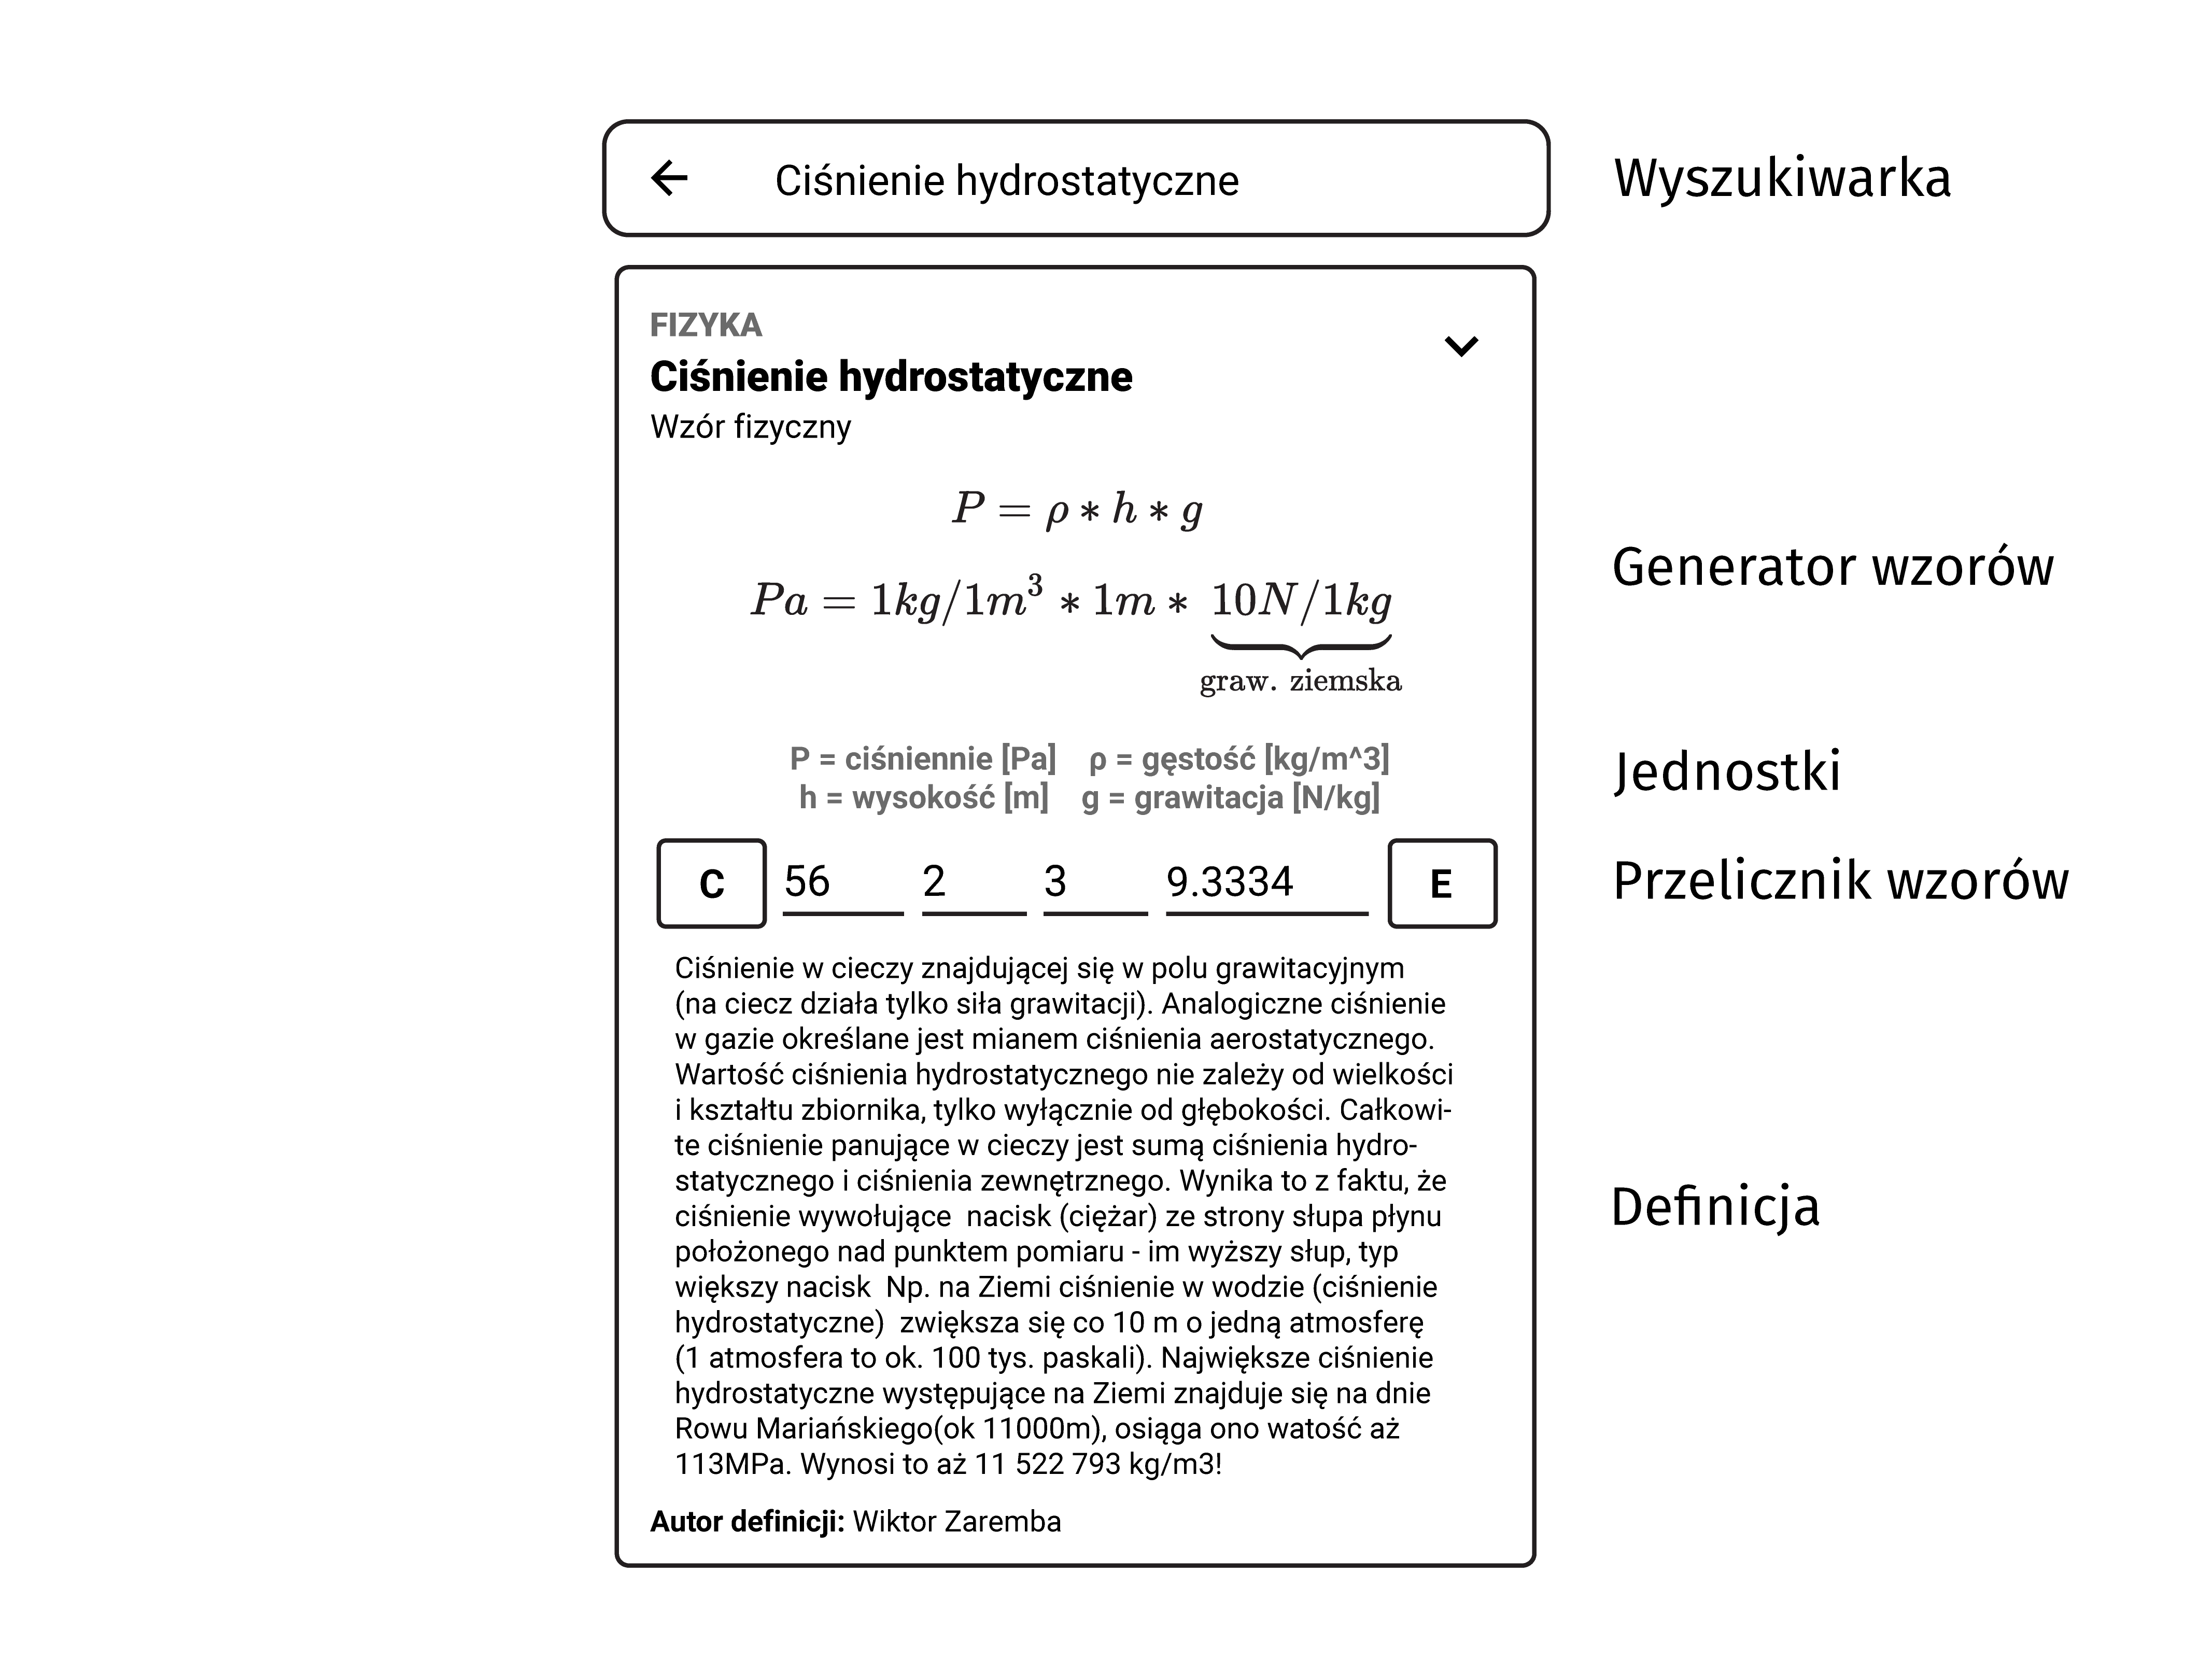
\includegraphics[width=10.5cm]{interfejs}
    \end{figure}
\end{frame}

\begin{frame}
	\tikzset{
	every shadow/.style={
		fill=none,
		shadow xshift=0pt,
		shadow yshift=0pt}
	}
  \smartdiagramset{
    circular distance=36mm,
    text width=80mm,
    font=\small,
    module minimum width=10mm,
    module minimum height=10mm,
    module shape=rectangle,
    uniform arrow color=true,
    arrow color=gray!50!black,
    border color=black,
    uniform color list=white for 6 items,
  }

  \frametitle{System nauki}
  	\begin{figure}[H]
  		\smartdiagram[flow diagram]{
		Pierwsza styczność z nowym zagadnieniem,
		Wykorzystywanie aplikacji przy wykonywaniu zadań,
 		Szybsze utrwalanie zagadnienia w praktyce,
 	   	Zrealizowanie materiału}
	\end{figure}

\end{frame}

\section{Doświadczenia}
\subsection{Przeprowadzenie testów w środowisku szkolnym}

\begin{frame}
\frametitle{Cele doświadczeń}
\begin{enumerate}
  \item Dowieść, że istnieją media internetowe, które wpływają korzystnie na proces przyswajania wiedzy
  \item Dowieść, że istnieją alternatywy dla platform social-learningowych
  \item Zaobserwować zachowania uczniów oraz ich oczekiwania wobec platform edukacyjnych
\end{enumerate}
\end{frame}

\begin{frame}
\frametitle{Sposób liczenia punktów}
\small
W doświadczeniu brały udział grupy dwu-, trzecio-, oraz czteroosobowe, dlatego brana pod uwagę jest ilość punktów przypadająca na jednego członka grupy.

$$\text{ilość punktów} = \frac{\text{długość lekcji (45min)} - \text{czas (w minutach)}}{ (\text{ilość błędów}+1) * \text{liczebność grupy}}$$

W dzieleniu dodawana jest wartość $+1$, aby uniknąć dzielenia przez $0$ w przypadku bezbłędnego rozwiązania wszystkich poleceń.

\textbf{Przykład:} Dwuosobowa grupa uczniów wykonała spośród czterech zadań matematycznych trzy dobrze. Niepoprawne wykonanie jednego zadania traktowane jest jako jeden błąd.

$$10.38 \approx \frac{45min - 3.5min}{ (1+1) * \text{2}}$$
\end{frame}


\begin{frame}
\frametitle{Średnia arytmetyczna wszystkich kategorii}

\begin{figure}[H]
	
\begin{tikzpicture}
	\begin{axis}
	[
	xbar,
	y axis line style = { opacity = 0 },
	axis x line       = none,
	tickwidth         = 0pt,
	enlarge y limits  = 0.2,
	enlarge x limits  = 0.02,
	nodes near coords,
	symbolic y coords = {Fizyka,Matematyka},
	legend style={at={(1,-0.2)},
	legend cell align={left},
	anchor=south west},
	ytick=data
	]
	\addplot coordinates { (21,Matematyka) (12.69,Fizyka) };
	\addplot coordinates { (10.38,Matematyka) (15.25,Fizyka) };
	\addplot coordinates { (4.37,Matematyka) (7.21,Fizyka) };
	\legend{Aplikacja, Internet, Kalkulator}
  \end{axis}
\end{tikzpicture}

\end{figure}
\end{frame}

\section{Wyniki}

\begin{frame}
b
\end{frame}

\section{Podsumowanie}

\begin{frame}
  \frametitle{Możliwe rozwiązanie problemu}
\end{frame}

\end{document}
